\documentclass{article}
\usepackage[utf8]{inputenc}
\usepackage{ gensymb }
\usepackage{ dsfont }
\usepackage{ polski }
\usepackage{ textcomp }
\usepackage{ amsmath }
\usepackage{ wasysym }
\usepackage{ amssymb }
\usepackage{natbib}
\usepackage{graphicx}
\usepackage{ dsfont }
\usepackage{xcolor}

\title{Combinatorics Problems in Polish}
\author{Andrzej "Mathinity" Kukla}
\date{ }
\begin{document}

\maketitle
\begin{flushleft}
\large \textbf{1a}. Ile dodatnich dzielników ma liczba $x=2\cdot3^4\cdot7^3\cdot11^2\cdot47^5\ ?$
\end{flushleft}
\normalsize{}

Każdy dodatni dzielnik x będzie iloczynem liczb pierwszych, które są dzielnikiem x. Stąd: $$y|x\Leftrightarrow y=2^{\epsilon_1}\cdot3^{\epsilon_2}\cdot7^{\epsilon_3}\cdot11^{\epsilon_4}\cdot47^{\epsilon_5},\quad \epsilon_j\in\mathds{N}\cup\{0\},\quad j\in\{1,...,5\}$$
z tym, że $\epsilon_1\leq1,\epsilon_2\leq4,\epsilon_3\leq3,\epsilon_4\leq2,\epsilon_5\leq5$. Z tego wynika, że x ma $2\cdot5\cdot4\cdot3\cdot6=720$ dodatnich dzielników.

\begin{flushleft}
\large \textbf{1b}. Ile dodatnich dzielników ma liczba $x= p_1^{\epsilon_1}\cdot p_2^{\epsilon_2}\dotsb p_n^{\epsilon_n}$, gdzie $p_i$ to różne liczby pierwsze?
\end{flushleft}
\normalsize{}

Analogicznie do zadania \textbf{1a.} wiemy, że liczba x ma $(\epsilon_1+1\cdot)(\epsilon_2+1)\dotsb(\epsilon_n+1)$ dodatnich dzielników.

\begin{flushleft}
\large \textbf{2a}. W pokerze, ile jest możliwości full'a (3+2)?
\end{flushleft}
\normalsize{}

Wybierzmy najpierw wartość, z której wybierzemy trójkę. Wartości mamy, 13, więc możliwości mamy \textbf{13}.

Następnie wybieramy, spośród 4 kart wybranej wartości 3 z nich, więc możliwości mamy $4 \choose 3$ = \textbf{4}.

W następnej kolejności wybieramy wartość, z której wybierzemy parę. Musi ona być inna niż poprzednia, więc możliwości mamy \textbf{12}.

Na sam koniec wybieramy, spośród 4 kart wybranej wartości 2 z nich, więc możliwości mamy $4 \choose 2$ = \textbf{6}.

Ostatecznie mamy $13\cdot4\cdot12\cdot6=$ \textbf{3744} możliwości full'a.

\begin{flushleft}
\large \textbf{2b}. W pokerze, ile jest możliwości koloru (5 tego samego koloru)?
\end{flushleft}
\normalsize{}

Wybierzmy najpierw kolor, możliwości mamy \textbf{4}.

Następnie wybieramy 5 kart spośród 13 dostępnych, więc możliwości mamy $13 \choose 5$ = \textbf{1287}

Na sam koniec od naszej liczby musimy odjąć ilość możliwych pokerów (ponieważ poker to także kolor), a pokerów jest \textbf{40}.

Ostatecznie mamy $4\cdot1284-40=$ \textbf{5108}

\begin{flushleft}
\large \textbf{3}. Ile jest możliwości posadzenia 6 mężczyzn i 6 kobiet przy okrągłym stole tak, aby siedzieli na przemian? Miejsca nie mają znaczenia, jedynie kto przy kim siedzi.
\end{flushleft}
\normalsize{}

Niech $X=1,2,3,4,5,6\}$ to będzie zbiór mężczyzn, a $Y=7,8,9,10,11,12\}$ to będzie zbiór kobiet. Tworząc ciąg:

$$x_1,y_1,x_2,y_2,x_3,y_3,x_4,y_4,x_5,y_5,x_6,y_6$$

i łącząc jego końce (tworząc cykl) stworzymy "wizualizację" okrągłego stołu.

Gdybyśmy nie tworzyli okrągłego stołu, a ludzi sadzalibyśmy przy prostokątnym stole przy jednej krawędzi to sprawa byłaby prosta, możliwości byłoby $6!\cdot6!=518400$. W przypadku okrągłego stołu problem komplikuje się.
Zauważmy, że ciąg
$$1,7,2,8,3,9,4,10,5,11,6,12$$
jest równy ciągowi
$$2,8,3,9,4,10,5,11,6,12,1,7$$
ponieważ po połączeniu obu końców i lekkim obróceniu "stołu" dostajemy to samo ułożenie (cykl, po przesunięciu cyklicznym jest równy pierwotnemu cyklowi: (123)=(231)). Widać, że takich równych sobie ciągów jest 6, więc dzieląc wynik dla "prostokątnego stołu" przez 6 otrzymamy żądany wynik: $$\frac{518400}{6}=259200$$ 

\begin{flushleft}
\large \textbf{4}. Ile jest możliwości posadzenia 8 osób przy okrągłym stole tak, aby pewne osoby X i Y nie siedziały obok siebie? Miejsca nie mają znaczenia, jedynie kto przy kim siedzi.
\end{flushleft}
\normalsize{}
Korzystając z rozważań z poprzedniego zadania, ustalmy następujący ciąg:
$$x_1,x_2,x_3,x_4,x_5,x_6,x_7,x_8$$

Ustawmy X na pierwszym miejscu (miejsce nie ma znaczenia, bo i tak można cyklicznym przesunięciem przestawić X na pierwsze miejsce). Wtedy na drugim oraz na ostatnim miejscu nie może pojawić się Y, bo Y nie może siedzieć obok X. Możemy więc wybrać \textbf{5} miejsc dla Y. Pozostałe osoby mogą siedzieć na dowolnych miejscach, więc mamy $5!=$ \textbf{120} możliwości na ich posadzenie. Ostateczny wynik to:

$$5*120=600$$

\begin{flushleft}
\large \textbf{5a}. Ile jest możliwości ustawienia 8 nierozróżnialnych wież na szachowej planszy tak, aby żadna nie mogła zaatakować żadnej innej?
\end{flushleft}
\normalsize{}

Ustawiając pierwszą wieżę mamy do dyspozycji $8\cdot8$ pól. Po ustawieniu pierwszej wieży zostaje nam $7\cdot7$ pól do ustawienia kolejnej wieży. Analogicznie idąc 8 wież (z uwzględnioną kolejnością wież) możemy ustawić na $8!^2$ sposobów. Wynik ten musimy jednak podzielić jeszcze przez liczbę możliwości ułożenia 8 wież w ciągu, ponieważ wieże mają być nierozróżnialne. Stąd ostateczny wynik to: $$\frac{8!^2}{8!}=8!=40320$$

\begin{flushleft}
\large \textbf{5b}. Ile jest możliwości ustawienia 8 nierozróżnialnych wież na planszy wymiarów $10\times10$ tak, aby żadna nie mogła zaatakować żadnej innej?
\end{flushleft}

Rozważając analogicznie do rozwiązania powyższego zadania możliwości będzie $10\cdot10\cdot9\cdot9\cdots4\cdot4\cdot3\cdot3=\frac{10!^2}{4}$, co także musimy podzielić przez liczbę możliwości ułożenia 8 wież w ciągu, więc ostateczny wynik to:
$$\frac{10!^2}{4\cdot8!}=5^2\cdot9\cdot9!=81648000$$



\begin{flushleft}
\large \textbf{6a}. Najkrótsza droga z $(0,0)$ do $(i,j)$ jest równa $i+j$. Ile jest takich dróg?
\end{flushleft}
\begin{center}
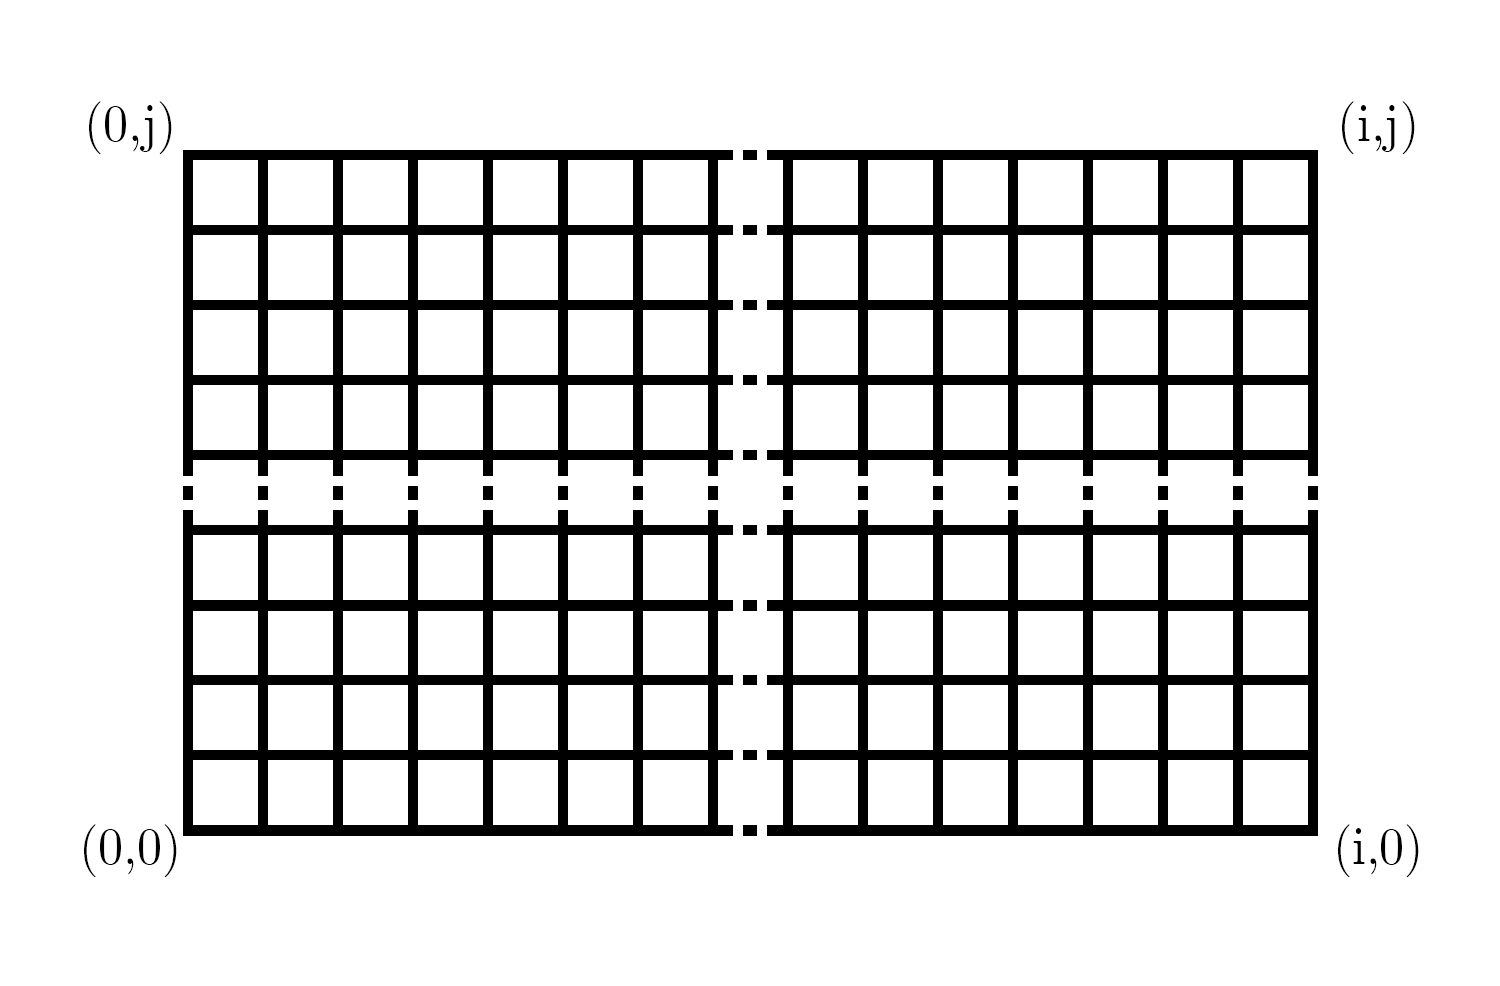
\includegraphics[scale=0.17]{path 1.jpg}
\end{center}

Popatrzmy na drogę jak na funkcję przyporządkowania. Mamy do wykonania $i+j$ ruchów, więc mamy $i+j$ pól do zapełnienia:
$$\underbrace{\_\ \_\ \_\ \_\ ...\ \_\ \_\ \_\ \_}_{i+j}$$ 

Każde pole zapełniamy ruchem na wschód albo na północ. Aby znaleźć liczbę różnych dróg najpierw przyporządkujmy do konkretnych pól wszystkie ruchy na wschód, czyli wybieramy i pól: $i+j\choose i$, a do pozostałych, pustych pól przypisujemy ruch na północ. Gdybyśmy najpierw przyporządkowywali do konkretnych pól wszystkie ruchy na północ, to byśmy wybierali j pól: $i+j\choose j$, ale 
$${{i+j}\choose{i} }={ {i+j}\choose{j}},$$
więc nie ma znaczenia które ruchy wybierzemy najpierw. 

Ostateczna odpowiedź to: $${{i+j}\choose{i} }$$

\begin{flushleft}
\large \textbf{6b}. Najkrótsza droga z $(0,0)$ do $(i,j)$ jest równa $i+j$. Załóżmy, że droga pomalowana na \textcolor{red}{czerwono} jest zamknięta. Ile jest najkrótszych dróg z $(0,0)$ do $(i,j)$ z pominięciem \textcolor{red}{czerwonej} drogi?
\end{flushleft}
\begin{center}
[Czerwona droga przebiega od punktu $(k,l)$ do punktu $(k,l+1)$]
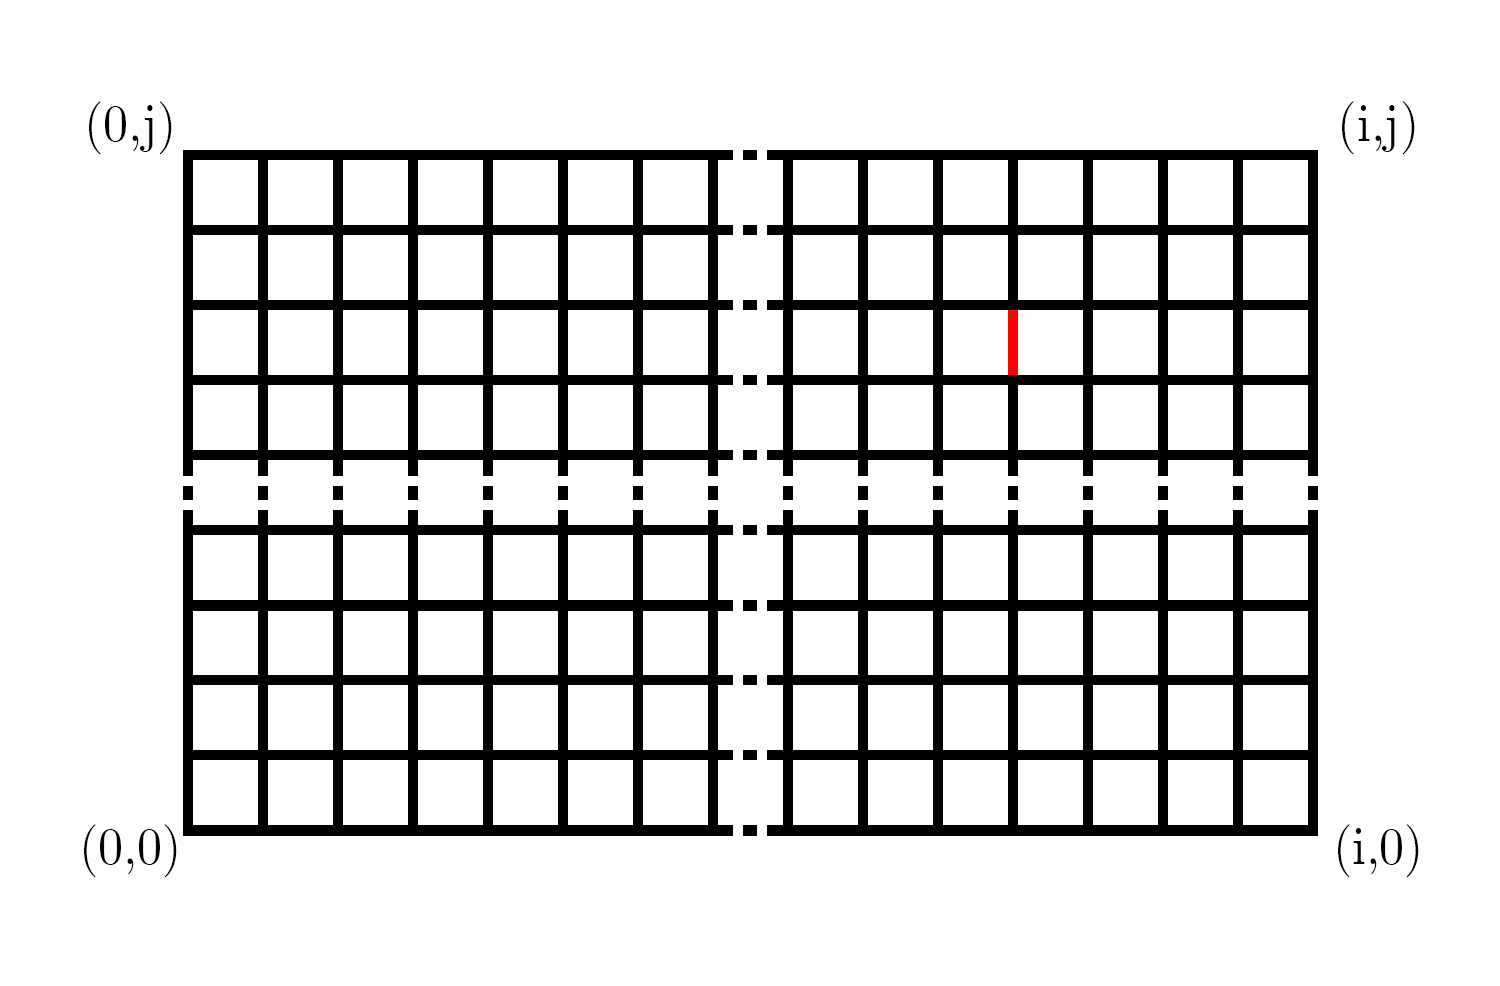
\includegraphics[scale=0.17]{path 2.jpg}
\end{center}

Aby policzyć, ile jest takich dróg weźmiemy wynik z 1a, czyli liczba wszystkich możliwych najkrótszych dróg i odejmiemy od niej te drogi, które przechodzą przez czerwoną drogę.

Aby droga przechodziła przez czerwoną drogę musi najpierw dotrzeć do jej dolnego krańca, czyli do punktu $(k,l)$, następnie przejść na punkt $(k,l+1)$ i stamtąd dotrzeć do punktu $(i,j)$. Powstają nam dwa obszary:
\begin{center}
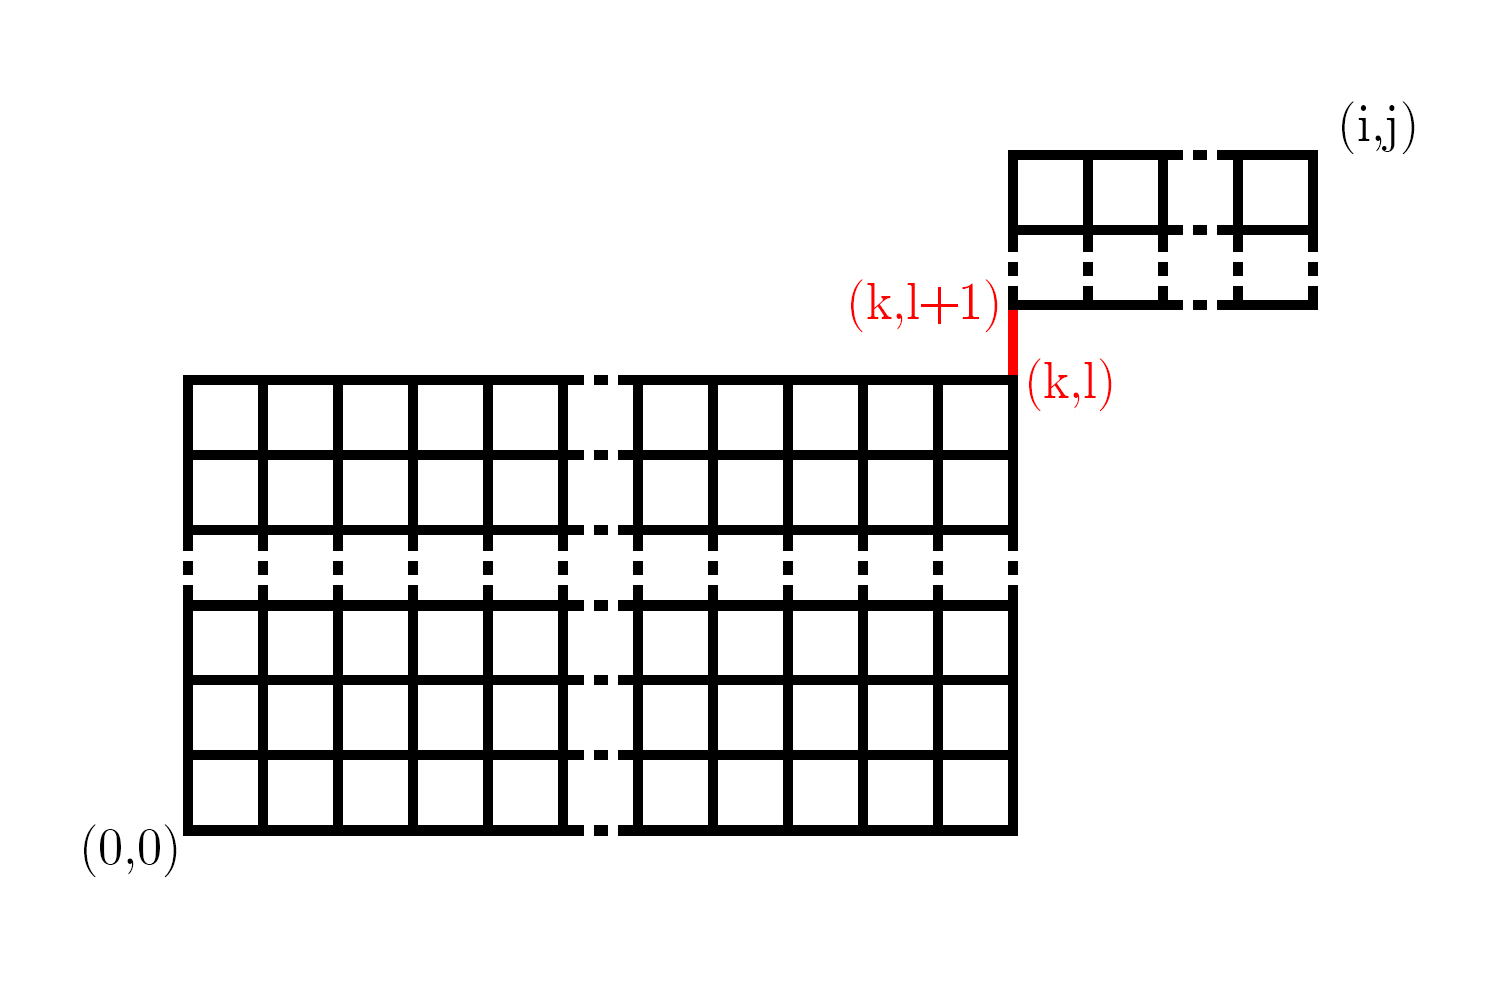
\includegraphics[scale=0.17]{path 3.jpg}
\end{center}

Mamy $k+l\choose k$ możliwych dróg na przejście z $(0,0)$ do $(k,l)$ (na podstawie rozwiązania 1a). Następnie, w trakcie każdej z tych dróg musimy przejść przez czerwoną drogę i ostatecznie mamy kolejnych $i+j-(k+l+1)\choose i-k$ możliwości przejścia do końca. Ostateczny wynik to:
$${{i+j}\choose{i} }-{k+l\choose k}\cdot{i+j-(k+l+1)\choose i-k}$$

\begin{flushleft}
\large \textbf{7}. Udowodnij kombinatorycznie (dla $m>n$,\quad $k<m,\quad k\leq n$) $$\sum_{i=0}^k {m\choose i}{n\choose k-i}={m+n\choose k}$$
\end{flushleft}
\textbf{DW.}
Wyobraźmy sobie, że musimy wybrać $k$ elementów ze zbioru $X$, którego moc to $m+n$ (prawa strona tezy). Podzielmy ten zbiór na dwa rozłączne podzbiory $X_1$ i $X_2$, których moce to odpowiednio $m$ i $n$, więc $X_1\cup X_2=X$. Aby wybrać $k$ elementów z $X$ możemy wybierać najpierw z $X_1$ pewną ilość elementów $i$, a następnie pozostałą ilość elementów $k-i$ wybrać ze zbioru $X_2$. Jeżeli wybierzemy $0$ elementów z $X_1$ (1 możliwość), to następnie musimy wybrać $k$ elementów z $X_2$ ($n\choose k$ możliwości). Jeżeli wybierzemy $1$ element z $X_1$ ($m\choose 1$ możliwości), to następnie musimy wybrać $k-1$ elementów z $X_2$ ($n\choose k-1$ możliwości). Analogicznie zwiększając liczbę elementów branych z $X_1$ otrzymamy k możliwości, które są wyczerpujące oraz rozłączne, a ich suma daje lewą stronę tezy, więc teza jest prawdziwa.
\begin{flushright}
$\blacksquare$
\end{flushright}

\textbf{(a)} Jeśli $m=n$, to 

$\cdot$ dla $k$ parzystego niech $l=\frac{k}{2}$

Wtedy wzór można zapisać w ten sposób:
$$2\cdot\sum_{i=0}^{l-1} {m\choose i}{m\choose k-i}+{m\choose l}^2={2m\choose k}$$

$\cdot$ dla $k$ nieparzystego niech $l=\frac{k-1}{2}$

Wtedy wzór można zapisać w ten sposób:
$$2\cdot\sum_{i=0}^{l} {m\choose i}{m\choose k-i}={2m\choose k}$$


\textbf{(b)} Jeśli $m=n=k$, a wiemy, że $${k \choose i}={k \choose k-i}$$

to wzór można zapisać w ten sposób:
$$\sum_{i=0}^k {k\choose i}^2={2k\choose k}$$


\begin{flushleft}
\large \textbf{8}. Załóżmy, że w pudełku mamy 18 piłek, gdzie każda z nich ma przypisany numerek, od 1 do 6, po 3 piłki na jeden numer. Ile jest możliwych rezultatów? 
\end{flushleft}

\textbf{(a)} Załóżmy, że kolejność wyciągania piłek ma znaczenie. Podzielmy to na przypadki:

\textbf{(1)} Pierwsze dwie piłki są takie same: 
\begin{itemize}
    \item Trzecia piłka jest taka sama jak poprzednie dwie. Wtedy mamy $6\cdot1\cdot1\cdot5$ możliwości.
    \item Trzecia piłka jest inna niż dwie poprzednie. Wtedy mamy $6\cdot1\cdot5\cdot6$ możliwości.
\end{itemize}

\textbf{(2)} Pierwsze dwie piłki są różne. Wtedy mamy $6\cdot5\cdot6\cdot6$ możliwości.

Ostatecznie mamy $30+180+1080=1290$ możliwości.

\textbf{(b)} Załóżmy, że kolejność wyciągania piłek nie ma znaczenia. Podzielmy to na przypadki:

\ 

\textbf{(1)} Wyciągnęliśmy 3 takie same piłki. Wtedy możliwości mamy $6\cdot5$

\textbf{(2)} Wyciągnęliśmy 2 pary piłek. Wtedy mamy $6\cdot5$ możliwości.

\textbf{(3)} Wyciągnęliśmy parę piłek, a pozostałe piłki się od nich różnią, a także różnią się miedzy sobą. Wtedy mamy $6\cdot5\cdot4$ możliwości.

\textbf{(4)} Każda piłka jest inna. Wtedy mamy $6\cdot5\cdot4\cdot3$ możliwości.

Ostatecznie mamy $30+30+120+360=540$ możliwości.

\begin{flushleft}
\large \textbf{9}. Ile jest permutacji słowa "Mississippi"?
\end{flushleft}

W słowie "Mississippi" mamy jedno "m", po cztery "s" i "i" i dwa "p". Permutacja musi się składać z 11 znaków. Zacznijmy od umieszczenia litery "m" w jednym z tych miejsc, mamy \textbf{11} możliwości. Następnie umieśćmy litery "s", mamy ${10\choose4}=$ \textbf{210} możliwości. Następnie umieśćmy litery "i", mamy ${6\choose4}=$ \textbf{15} możliwości. Litery "p" wstawiamy w pozostałe miejsca. Tym sposobem otrzymujemy $11\cdot210\cdot15=$ \textbf{34650} permutacji.

\begin{flushleft}
\large \textbf{10}. Znajdź liczbę całkowitych rozwiązań równania 
$$x_1+x_2+x_3+x_4+x_5=50$$
dla $x_1\geq -3,x_2\geq0,x_3\geq4,x_4\geq2,x_5\geq12$.
\end{flushleft}
Przekształćmy to równanie tak, aby dolne granice naszych równań były równe 0:
$$y_1=x_1+3,y_2=x_2,y_3=x_3-4,y_4=x_4-2,y_5=x_5-12$$
Podstawiając "igreki" za "iksy" otrzymujemy następujące równanie:
$$y_1+y_2+y_3+y_4+y_5=35$$
dla $y_i\geq0$, gdzie $i\in \{1,2,3,4,5\}$.

Otrzymujemy następującą liczbę całkowitych rozwiązań "igrekowego" równania: 
$${35+5-1\choose35}={39\choose35},$$
która jest także liczbą całkowitych rozwiązań oryginalnego równania.
\end{document}